\chapter {Resultados}
\par En esta sección se exponen los aspectos más destacados de la solución construida.

\section{Facilidad de despliegue}
\par La solución es fácilmente desplegable en entornos Kubernetes. Para ello, sólo será necesario realizar los siguientes pasos:
\begin{enumerate}
  \item Descargar repositorio: \\
		\begin{minipage}{\linewidth}
		\begin{lstlisting}[language=bash]
git clone git@github.com:bpk667/CircumCaetera.git
		\end{lstlisting}
		\end{minipage}
  \item Definir parámetros del entorno. \\
		\begin{minipage}{\linewidth}
		\begin{lstlisting}[language=bash]
DOMAIN="example.org"                          # Domain for the web services.
OWNER="$(whoami)"                             # Ownner of the Docker registry.
EMAIL="example@protonmail.com"                # Required by Let's Encrypt.
CERTIFICATEPATH="/exports/certs/${DOMAIN}"    # Host NFS repository for sharing certificates.
REGISTRY="localhost:5000"                     # Docker registry.
NFSSERVER="NFS_SERVER_IP"                     # IP of the NFS server
		\end{lstlisting}
		\end{minipage}
  \item Desplegar la aplicación. \\
		\begin{minipage}{\linewidth}
		\begin{lstlisting}[language=bash]
CircumCaetera/scripts/cc_deployWAF.sh
		\end{lstlisting}
		\end{minipage}
\end{enumerate}

No obstante, este despliegue tiene como requisitos que los registros DNS y el recurso NFS hayan sido previamente configurados.

\section{Adaptabilidad de la solución}
\par Dado que todo el proyecto está licenciado con licencia \acrlong{gpl} versión 3, cualquier que necesite modificar la solución puede hacerlo.
\par Por otro lado, toda la solución ha sido diseñada de forma modular con el fin de facilitar su uso parcial en los entornos en los que así se requiera. Algunos ejemplos de casos de uso en los que se utilice algún componente de la solución: 
\begin{itemize}
\item Se requiere implementar TLS adecuadamente, pero no se quieren utilizar los componentes WAF.
\item Se quiere desplegar WAF+TLS en un entorno Docker con un orquestador diferente.
\item Se quiere desplegar la solución WAF+TLS sin el gestor de certificados debido a que se dispone de una CA propia.
\end{itemize}

\section{Controles adicionales}
\par Se han implementado una serie de controles adicionales que no son estrictamente competencia de un WAF, como son la mejora de en la seguridad de las cookies, las cabeceras de seguridad o forzar el uso de canales
cifrados mediante la cabecera \cite{wiki:hsts}.
\par Adicionalmente, se ha configurado un gestor de certificados que permite implementar HTTPS de forma sencilla para el usuario.

\section{Validación de la seguridad}
Para poder validar la seguridad ofrecida por la solución, se ha escaneado la plataforma con las siguientes herramientas:
\par {\em Qualys. SSL Labs~\cite{ssllabs}}. Se trata de una herramienta online que ejecuta una batería de pruebas con el objetivo de verificar la seguridad de la página web.
\par En la figura ~\hyperref[tabla:resumenqualys]{Resumen ejecutivo de Qualys SSL Labs} se puede ver un resumen del resultado de las pruebas. En el apéndice
(~\hyperref[tabla:informequalys]{Informe completo de Qualys} ) se puede leer el informe completo.

\begin{figure}[!ht]
  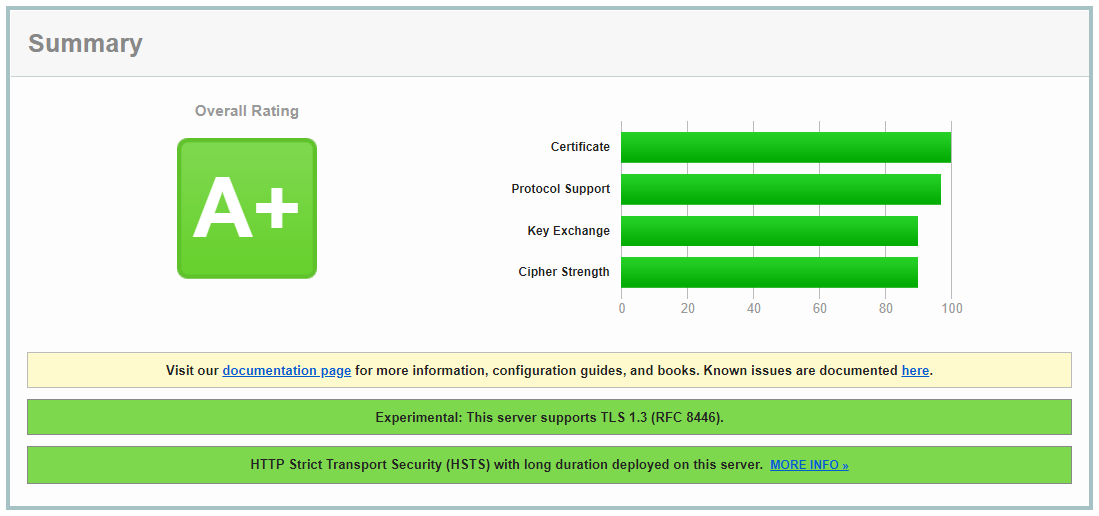
\includegraphics[width=0.9\textwidth]{fig/SSLTLS_Report_Summary}
  \label{tabla:resumenqualys}
  \caption{Resumen ejecutivo de Qualys SSL Labs}
\end{figure}
\par Entre otros, los test ejecutados incluyen: Configuración TLS, vulnerabilidades TLS y configuración de certificados.

\par Otra herramienta online que se ha ejecutado es {\em Security Headers} de Netsparker~\cite{securityheaders}.
\par En la figura ~\hyperref[tabla:resumensecurityheaders]{Resumen ejecutivo de Security Headers} se puede ver un resumen del resultado de las pruebas. En el apéndice
(~\hyperref[tabla:informesecurityheaders]{Informe completo de Security Headers} ) se puede leer el informe completo.

\begin{figure}[!ht]
  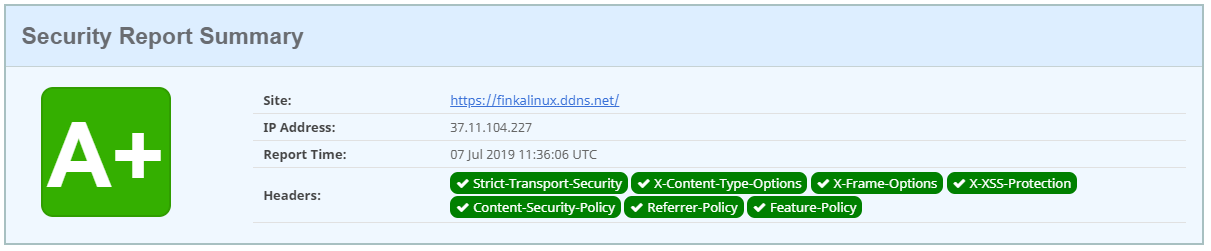
\includegraphics[width=0.9\textwidth]{fig/SecurityHeaders_Report_Summary}
  \label{tabla:resumensecurityheaders}
  \caption{Resultados cabeceras HTTP de seguridad}
\end{figure}
Entre otros, los test ejecutados incluyen: {\em \acrlong{hsts}} (\acrshort{hsts}), {\em X-XSS-Protection}, {\em Content-Security-Policy} o la reciente {\em Feature-Policy}.

